\documentclass[journal]{IEEEtran}

\usepackage{cite}
\usepackage{amsmath,amssymb,amsfonts}
\usepackage{graphicx}
\usepackage{textcomp}
\usepackage{booktabs}
\usepackage{array}
\usepackage{tabularx}
\usepackage{float}
\usepackage{pgfplots}
\pgfplotsset{compat=1.16}
\usepackage[hidelinks]{hyperref}

\newcolumntype{Y}{>{\raggedright\arraybackslash}X}

\begin{document}

\title{Comparison of the Qiskit, PennyLane and Cirq Quantum Software Development Kits}

\author{\IEEEauthorblockN{Swati Ghosh}
\IEEEauthorblockA{B.Tech CS \& AI, Newton School of Technology, Rishihood University\\
Sonipat, India\\
ghshswt@gmail.com}}

\maketitle

\begin{abstract}
Software development kits can be utilised by developers to design, optimise and run quantum algorithms. Here we compare three popular open source quantum development kits: Qiskit, PennyLane and Cirq. We consider the ease-of-use of each, alongside their simulation performance and quantum machine learning and quantum-classical hybrid functionality. Each development kit is used to programme and run (on local simulators) equivalent quantum algorithms. Specifically, these include the Bell state, Grover's search algorithm, the Quantum Fourier Transform and a parametric quantum circuit. Our comparison finds that, of the three, Qiskit offers the most comprehensive general-purpose development environment and has the most tools available. PennyLane excels in quantum machine learning and quantum-classical hybrid functionality. Furthermore, Cirq is well suited to quantum circuit research and includes functionality for device-aware circuit design. Depending on a user's requirement, then, Qiskit is most appropriate for general quantum development, PennyLane for quantum machine learning and Cirq for circuit research.
\end{abstract}

\begin{IEEEkeywords}
Quantum computing, Qiskit, PennyLane, Cirq, quantum software development kit, quantum simulation, comparison.
\end{IEEEkeywords}

%==================================================================
\section{Introduction}
Quantum computers exploit quantum physics principles e.g, superposition and entanglement, to potentially exceed classical computers in some areas of computation. Alongside continual advancement in quantum hardware, there has been increased development of quantum software to facilitate the transformation of quantum algorithms into circuits.

The Qiskit, PennyLane and Cirq development kits are all popular quantum Python based software. IBM developed Qiskit which is a general purpose quantum software development kit offering design, optimisation, simulation and running of quantum circuits. PennyLane, developed by Xanadu, specialises in quantum machine learning, automatic differentiation and quantum-classical hybrid function. Finally, Cirq, created by Google Quantum AI, is used for quantum circuit design and simulation with a focus on device-aware functionality.

Whilst all three development kits can be used for quantum circuit design, they differ in terms of their functionality, back-ends and target audience. Consequently, it is important to compare them so as to identify the most suitable development kit for education, research and/or industry.

\subsection{Research Questions}
This research investigates:
\begin{enumerate}
\item How do the syntax and ease-of-use of these development kits differ?
\item How do the development kits compare in terms of simulation performance?
\item Which development kit offers the best quantum machine learning and quantum-classical hybrid functionality?
\item What are the main differences in terms of device back-end access, documentation and ecosystem provision?
\item Which development kit is most appropriate for novices, for researchers and for quantum machine learning developers?
\end{enumerate}

\subsection{Objectives}
Our research aims to:
\begin{enumerate}
\item Compare key aspects for each development kit.
\item Program and run equivalent quantum algorithms using all three.
\item Investigate the simulation performance in terms of time, memory and circuit depth and analyse the effort associated with the programmes.
\item Assess documentation, ease of installation and device access.
\item Provide guidance on suitable development kits for various user groups.
\end{enumerate}

\subsection{Contributions}
This paper makes the following contributions:
\begin{enumerate}
\item A comparison of the development kit's key features.
\item Benchmarking for selected quantum algorithms.
\item Guidance for novices, researchers and developers on suitable development kits.
\item Analysis of the benefits and challenges of each development kit.
\end{enumerate}

%==================================================================
\section{Literature Review}

\subsection{Quantum Development Kits}
Quantum development kits contain functionality relating to qubits, gates, circuits and measurement. In addition, they can interface with simulators and devices. These allow developers to program quantum computers at the circuit level and thus simplify the programming process.

\subsection{Qiskit}
Qiskit is an open-source quantum development kit that was initially developed by IBM and is based on Python. It can be used to programme, optimise and simulate quantum circuits and also run them on IBM Quantum devices. It is widely utilised for quantum education and research. There is also a large quantity of supporting documentation, libraries and community resources. The 2026 Unitary Foundation survey noted that Qiskit was the most widely used full-stack quantum development kit and simulator, with 56.8\% of respondents either currently or planning to use it.

\subsection{PennyLane}
PennyLane is an open source, cross-platform quantum development kit that is specialised for quantum machine learning, automatic differentiation and optimisation of quantum-classical hybrid function. It can programme quantum circuits for a variety of back-ends and has plugins for both Qiskit and Cirq. PennyLane's ability to calculate gradients makes it highly suitable for quantum algorithms, quantum chemistry and machine learning.

\subsection{Cirq}
Cirq is an open-source quantum development kit, also based on Python, which was developed by Google Quantum AI. This enables quantum circuits to be programmed, manipulated and simulated. Again, there is an emphasis on device-aware functionality and fine control of circuits. Cirq is particularly relevant for quantum researchers wishing to programme for and conduct research on noisy intermediate-scale quantum devices, together with those who desire high levels of circuit control.

\subsection{Research Gap}
Whilst information is often given on an individual basis for each development kit, there is infrequently a comparative investigation of PennyLane, PennyLane and Cirq which analyses equivalent quantum circuits, utilises similar assessment criteria and is undertaken within a common development environment. This paper tackles this issue by combining comparative analysis and benchmarking.

%==================================================================
\section{Methodology}

\subsection{Research Approach}
Our research adopts a mixed methods approach and includes:
\begin{enumerate}
\item Analysis of documentation and functionality.
\item Quantitative benchmarking of quantum circuits.
\item Assessment of ease-of-use, which incorporates programme effort and documentation quality.
\end{enumerate}

\subsection{Development Kits Reviewed}
\begin{table}[!t]
\caption{Development Kits Reviewed}
\label{tab:kits}
\centering
\small
\begin{tabularx}{\columnwidth}{l l Y}
\toprule
\textbf{Platform} & \textbf{Maintainer} & \textbf{Primary focus}\\
\midrule
Qiskit & IBM & Generic quantum\\
PennyLane & Xanadu & Quantum machine learning and hybrid\\
Cirq & Google Quantum AI & Circuit design and quantum research\\
\bottomrule
\end{tabularx}
\end{table}

\subsection{Test Environment}
Computing specifications included:
\begin{itemize}
\item Python: 3.13.18
\item Platform: Linux-6.6.159+-x86\_64-with-glibc2.39
\item Qiskit: 2.6.2
\item PennyLane: 0.45.1
\item Cirq: 1.7.0
\item CPU: x86\_64
\end{itemize}
Each quantum circuit was run a number of times, and the mean time was determined in order to minimise the impact of random factors.

\subsection{Comparison Factors}
The following factors were analysed for comparison:
\begin{itemize}
\item Installation and configuration
\item Syntax
\item Simulation performance
\item Memory usage
\item Circuit depth and gate numbers
\item Quantum machine learning functionality
\item Device and back-end access
\item Documentation and education materials
\item Community and ecosystem
\item Programme clarity and effort
\end{itemize}

\subsection{Quantum Circuits Investigated}
The following circuits were analysed as they are commonly encountered in education, algorithm and quantum machine learning contexts:

\begin{table}[!t]
\caption{Quantum Circuits Investigated}
\label{tab:circuits}
\centering
\small
\begin{tabularx}{\columnwidth}{l Y}
\toprule
\textbf{Circuit} & \textbf{Function}\\
\midrule
Bell state & Examines entanglement and measurement\\
Quantum Fourier Transform & Investigates organised gate application\\
Variational quantum circuit & Analyses parametric circuits and gradient calculation\\
Grover's search & Analyses quantum iterative search\\
\bottomrule
\end{tabularx}
\end{table}

\subsection{Performance Indicators}
Information was gathered on:
\begin{enumerate}
\item Execution time: Time taken to run a quantum circuit (mean wall-clock time).
\item Memory usage: Maximum memory usage.
\item Circuit depth: Number of gate strata (circuit depth).
\item Gate count: Number of gates.
\item Lines of code: Number of program lines.
\item Result accuracy: Degree of alignment between simulated and theoretical outcomes.
\end{enumerate}

%==================================================================
\section{Results}

\subsection{Functional Comparison}
\begin{table*}[!t]
\caption{Functional Comparison of Qiskit, PennyLane and Cirq}
\label{tab:functional}
\centering
\small
\begin{tabularx}{\textwidth}{l Y Y Y}
\toprule
\textbf{Factor} & \textbf{Qiskit} & \textbf{PennyLane} & \textbf{Cirq}\\
\midrule
Target & Generic quantum & Generic quantum machine learning and optimisation & Quantum circuit research and device-aware\\
Language & Python & Python & Python\\
Syntax & High level and adaptable & High level -- with an ML focus & High level -- with a research focus\\
Simulator & Excellent with Aer simulator & Multi-backend plugin functionality & Excellent built-in simulators\\
Quantum machine learning & Available & Excellent built-in functionality & Minimal without plugins\\
Device and backend access & IBM Quantum and other back-ends & Multi-backend plugin functionality & Google-focused ecosystem and plugins\\
Documentation & Voluminous & Excellent for quantum machine learning & Research focused\\
Community and ecosystem & Largest & Currently rapidly expanding & Excellent research community\\
\bottomrule
\end{tabularx}
\end{table*}

PennyLane can utilise the Qiskit and Cirq back-ends via plugins and is hence cross-platform.

\subsection{Benchmarking Data}
Table~\ref{tab:time} lists the mean simulation times for each circuit and framework, and Fig.~\ref{fig:time} compares them graphically.

\begin{table}[!t]
\caption{Mean Simulation Times (ms)}
\label{tab:time}
\centering
\footnotesize
\setlength{\tabcolsep}{3pt}
\begin{tabularx}{\columnwidth}{Y l r r}
\toprule
\textbf{Circuit} & \textbf{Framework} & \textbf{Mean Time (ms)} & \textbf{Std Dev (ms)}\\
\midrule
Bell state & Qiskit & 0.834020 & 1.088765\\
Bell state & PennyLane & 3.570422 & 3.578012\\
Bell state & Cirq & 0.736945 & 0.144340\\
\midrule
Grover's search & Qiskit & 1.748815 & 0.085610\\
Grover's search & PennyLane & 4.398296 & 0.376946\\
Grover's search & Cirq & 5.355646 & 0.902332\\
\midrule
Quantum Fourier Transform & Qiskit & 0.894576 & 0.088148\\
Quantum Fourier Transform & PennyLane & 0.884073 & 0.096977\\
Quantum Fourier Transform & Cirq & 2.139373 & 0.187327\\
\midrule
Variational circuit & Qiskit & 1.209801 & 0.231337\\
Variational circuit & PennyLane & 3.514917 & 0.641212\\
Variational circuit & Cirq & 2.793939 & 0.380610\\
\bottomrule
\end{tabularx}
\end{table}

\begin{figure}[!t]
\centering
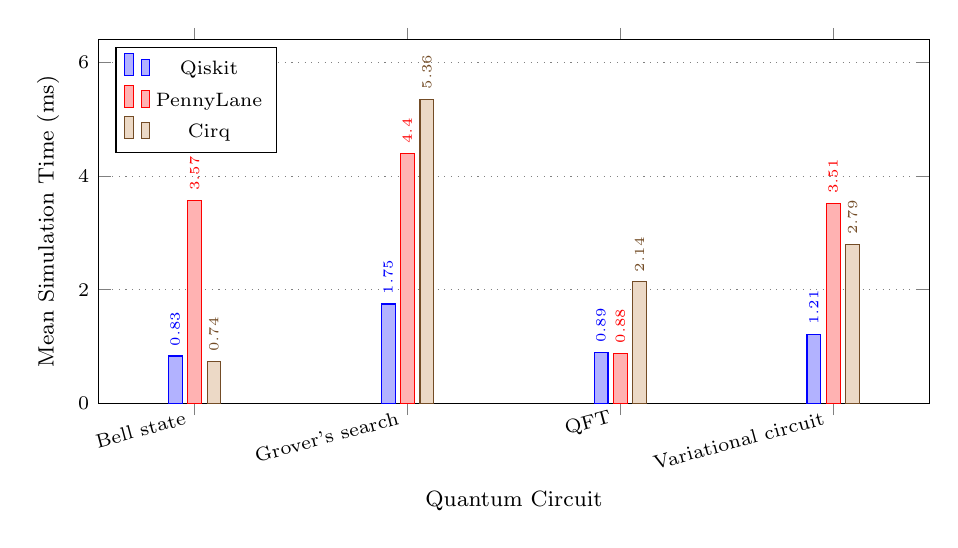
\begin{tikzpicture}
\begin{axis}[
    ybar,
    width=\columnwidth,
    height=6.2cm,
    bar width=5pt,
    ymin=0, ymax=6.4,
    ylabel={Mean Simulation Time (ms)},
    xlabel={Quantum Circuit},
    symbolic x coords={Bell state,Grover's search,QFT,Variational circuit},
    xtick=data,
    xticklabel style={font=\scriptsize, rotate=15, anchor=east},
    yticklabel style={font=\scriptsize},
    label style={font=\footnotesize},
    legend style={font=\scriptsize, at={(0.02,0.98)}, anchor=north west},
    nodes near coords,
    nodes near coords style={font=\tiny, rotate=90, anchor=west, /pgf/number format/.cd, fixed, precision=2},
    enlarge x limits=0.15,
    ymajorgrids, grid style={dotted,gray}
]
\addplot coordinates {(Bell state,0.834020) (Grover's search,1.748815) (QFT,0.894576) (Variational circuit,1.209801)};
\addplot coordinates {(Bell state,3.570422) (Grover's search,4.398296) (QFT,0.884073) (Variational circuit,3.514917)};
\addplot coordinates {(Bell state,0.736945) (Grover's search,5.355646) (QFT,2.139373) (Variational circuit,2.793939)};
\legend{Qiskit,PennyLane,Cirq}
\end{axis}
\end{tikzpicture}
\caption{Mean simulation time comparison of Qiskit, PennyLane and Cirq for each quantum circuit (QFT: Quantum Fourier Transform).}
\label{fig:time}
\end{figure}

Table~\ref{tab:loc} and Fig.~\ref{fig:loc} report the program effort in lines of code.

\begin{table}[!t]
\caption{Program Effort (Number of Lines)}
\label{tab:loc}
\centering
\small
\begin{tabular}{l r r r}
\toprule
\textbf{Circuit} & \textbf{Qiskit} & \textbf{PennyLane} & \textbf{Cirq}\\
\midrule
Bell state & 5 & 8 & 6\\
Grover's search & 20 & 23 & 18\\
Quantum Fourier Transform & 10 & 7 & 3\\
Variational circuit & 10 & 13 & 11\\
\bottomrule
\end{tabular}
\end{table}

\begin{figure}[!t]
\centering
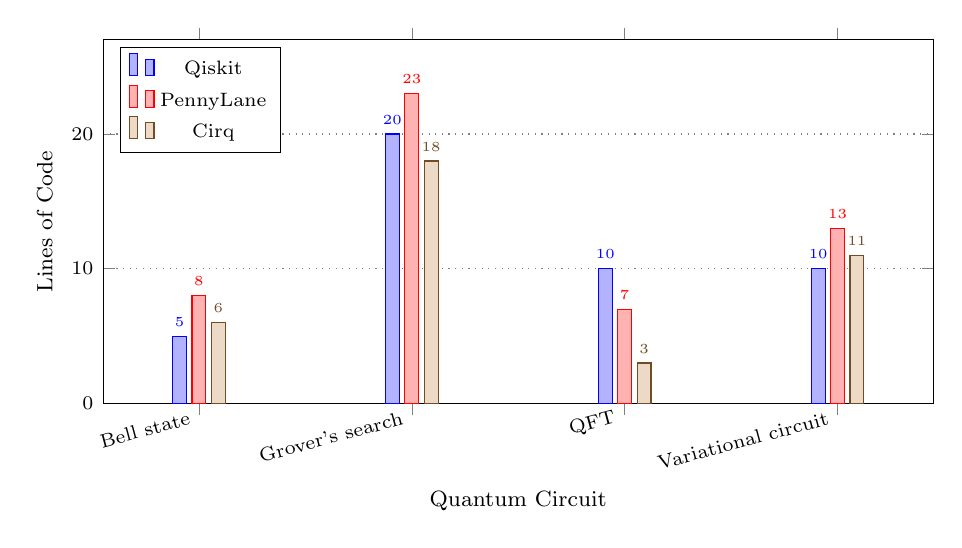
\begin{tikzpicture}
\begin{axis}[
    ybar,
    width=\columnwidth,
    height=6.2cm,
    bar width=5pt,
    ymin=0, ymax=27,
    ylabel={Lines of Code},
    xlabel={Quantum Circuit},
    symbolic x coords={Bell state,Grover's search,QFT,Variational circuit},
    xtick=data,
    xticklabel style={font=\scriptsize, rotate=15, anchor=east},
    yticklabel style={font=\scriptsize},
    label style={font=\footnotesize},
    legend style={font=\scriptsize, at={(0.02,0.98)}, anchor=north west},
    nodes near coords,
    nodes near coords style={font=\tiny},
    enlarge x limits=0.15,
    ymajorgrids, grid style={dotted,gray}
]
\addplot coordinates {(Bell state,5) (Grover's search,20) (QFT,10) (Variational circuit,10)};
\addplot coordinates {(Bell state,8) (Grover's search,23) (QFT,7) (Variational circuit,13)};
\addplot coordinates {(Bell state,6) (Grover's search,18) (QFT,3) (Variational circuit,11)};
\legend{Qiskit,PennyLane,Cirq}
\end{axis}
\end{tikzpicture}
\caption{Program effort (lines of code) comparison of Qiskit, PennyLane and Cirq for each quantum circuit (QFT: Quantum Fourier Transform).}
\label{fig:loc}
\end{figure}

\begin{table}[!t]
\caption{Circuit Depth and Gates}
\label{tab:depth}
\centering
\footnotesize
\setlength{\tabcolsep}{3pt}
\begin{tabularx}{\columnwidth}{Y l r r}
\toprule
\textbf{Circuit} & \textbf{Framework} & \textbf{Circuit Depth} & \textbf{Gate Count}\\
\midrule
Bell state & Qiskit & 2 & 2\\
Bell state & PennyLane & 2 & 2\\
Bell state & Cirq & 2 & 2\\
\midrule
Grover's search & Qiskit & 21 & 43\\
Grover's search & PennyLane & 21 & 43\\
Grover's search & Cirq & 21 & 43\\
\midrule
Quantum Fourier Transform & Qiskit & 8 & 12\\
Quantum Fourier Transform & PennyLane & 1 & 1\\
Quantum Fourier Transform & Cirq & 1 & 1\\
\midrule
Variational circuit & Qiskit & 9 & 22\\
Variational circuit & PennyLane & 9 & 22\\
Variational circuit & Cirq & 9 & 22\\
\bottomrule
\end{tabularx}
\end{table}

\subsection{Ease-of-Use Analysis}
Generally, Qiskit contains good instructional, visualisation and example resources. PennyLane although slightly more complex to initially understand due to its specialisation in quantum machine learning, has excellent facilities for gradient and optimisation calculation. Meanwhile, Cirq, although offering excellent circuit control, may involve greater hands-on programme design for higher-level functionality.

%==================================================================
\section{Discussion}

\subsection{Syntax}
All three development kits can be used to program in Python. If a general-purpose development kit is required, then Qiskit is a suitable choice. PennyLane is most easily used where circuits are to be trained and/or optimised using classical machine learning techniques. Likewise, Cirq is a good option for quantum researchers desiring high circuit and device control.

\subsection{Simulation Performance}
Results have shown that different quantum circuits and frameworks can lead to varying degrees of simulation efficiency. Out of the three frameworks, Qiskit had the most efficient simulations. It was quickest at simulating both Grover's search and the variational circuit (with times of 1.74882 ms and 1.20980 ms, respectively). Cirq was most efficient for simulating the Bell state (time taken = 0.73695 ms), and PennyLane was most efficient for simulating the Quantum Fourier Transform (time taken = 0.88407 ms), marginally quicker than Qiskit (time taken = 0.89458 ms).

Furthermore, Grover's search was found to take the most simulation time to run in comparison to the other circuits on all three frameworks. Cirq had the longest simulation time for this circuit (5.35565 ms), whereas Qiskit took 1.74882 ms. This therefore suggests that a framework's efficiency is influenced by both the nature of the circuit being simulated and its implementation.

Generally, Cirq needed less code to implement the circuits investigated. It took 6, 18, 3 and 11 lines of code to simulate the Bell state, Grover's search, QFT and variational circuits respectively. Both the Bell state and variational circuits were also implemented using less code on Qiskit. However, PennyLane did not use the least amount of code to simulate either of these. Thus, it appears that both the type of circuit and the programming constructs available within a framework can affect the coding effort that is needed.

Taken as a whole, there does not appear to be one framework that is always most efficient in all aspects. Although Qiskit had good simulation efficiency, Cirq generally involved less coding effort, and PennyLane had good simulation efficiency for the QFT. Hence, when deciding on which framework to utilise, factors such as simulation efficiency, coding effort and the circuit and application in question should all be considered.

\subsection{Quantum Machine Learning}
As it is designed for differentiable quantum circuits and quantum-classical hybrid functions, PennyLane is most effective for quantum machine learning. Further, PennyLane can interface with both Qiskit and Cirq via plugins and so a user can therefore utilise PennyLane's quantum machine learning functionality with the back-ends of these other development kits.

\subsection{Device and Back-End}
In terms of general availability, Qiskit has the most extensive ecosystem, particularly for those wishing to program for IBM Quantum. PennyLane also demonstrates good versatility through its multi-backend plugin functionality. Finally, Cirq is especially useful for quantum researchers wanting to programme for, and research on, Google-orientated quantum devices, as well as for those requiring high circuit control.

\subsection{Recommendations}
\begin{table}[H]
\caption{Recommended Development Kit by User Type}
\label{tab:recs}
\centering
\footnotesize
\setlength{\tabcolsep}{3pt}
\begin{tabularx}{\columnwidth}{>{\raggedright\arraybackslash}p{2.1cm} >{\raggedright\arraybackslash}p{1.9cm} Y}
\toprule
\textbf{User type} & \textbf{Recommended development kit} & \textbf{Reason}\\
\midrule
Novice & Qiskit & Good instruction, visualisation and education resources are available.\\
Quantum machine learning developer & PennyLane & Built-in gradient and hybrid functionality are available.\\
Quantum device researcher & Cirq & High circuit and device control is achievable.\\
General purpose developer & Qiskit & There is a wide range of resources and tools that are well established.\\
Cross-platform development developer & PennyLane & It can interface with both the Qiskit and Cirq back-ends.\\
\bottomrule
\end{tabularx}
\end{table}

%==================================================================
\section{Limitations}
There are several constraints to our research. Firstly, our benchmarking was undertaken on one computer, and so results may vary on different hardware. Secondly, only four example quantum circuits were analysed. Thirdly, we utilised local simulators and did not run our program on actual quantum devices. Finally, our results are specific to the particular versions of Qiskit, PennyLane and Cirq that were analysed. Moreover, our evaluation of documentation was subjective and based on our own judgement of ease-of-use.

%==================================================================
\section{Conclusion and Further Work}
We compared the ease of use, simulation performance, quantum machine learning functionality, device access and ecosystem provision for the Qiskit, PennyLane and Cirq quantum development kits. Our analysis shows that there is no universally optimal development kit. Rather, Qiskit is best for general quantum development, PennyLane for quantum machine learning, and Cirq for quantum circuit research.

Further work should build upon our research. Firstly, additional quantum algorithms could be analysed such as Shor's algorithm and quantum error correction circuits. Secondly, performance could be investigated on real quantum devices. Thirdly, noise tolerance could be assessed. Finally, further development kits such as Amazon Braket and TKET could be compared.

%==================================================================
\nocite{*}
\begin{thebibliography}{1}
\bibitem{qiskitdoc}
IBM Quantum, ``Qiskit Documentation.'' [Online]. Available: \url{https://www.ibm.com/quantum/qiskit}

\bibitem{qiskitgh}
Qiskit Development Team, ``Qiskit GitHub.'' [Online]. Available: \url{https://github.com/Qiskit/qiskit}

\bibitem{pldoc}
Xanadu, ``PennyLane Documentation.'' [Online]. Available: \url{https://docs.pennylane.ai/en/stable}

\bibitem{cirqdoc}
Google Quantum AI, ``Cirq Documentation.'' [Online]. Available: \url{https://quantumai.google/cirq}

\bibitem{unitary}
Unitary Foundation, ``2026 Quantum Open Source Software Survey Results.'' [Online]. Available: \url{https://unitary.foundation/posts/2026_survey_results/}

\bibitem{plqiskit}
``PennyLane-Qiskit Plugin Documentation.'' [Online]. Available: \url{https://docs.pennylane.ai/projects/qiskit/en/stable/}

\bibitem{plcirq}
``PennyLane-Cirq Plugin Documentation.'' [Online]. Available: \url{https://docs.pennylane.ai/projects/cirq/en/latest/}
\end{thebibliography}

\end{document}